\documentclass[11pt]{article}
\usepackage{./styles/daves,fancyhdr,natbib,url}
\usepackage{amsmath,amssymb,caption,graphicx,pdfpages,lscape}
\usepackage{booktabs}
\usepackage{dcolumn}


\DeclareGraphicsRule{.tif}{png}{.png}{`convert #1 `dirname #1`/`basename #1 .tif`.png}
\thispagestyle{plain}
\bibliographystyle{./styles/chicago}
%\bibliographystyle{apalike}
\lhead{CE 5333}
\rhead{SPRING 2020}
\lfoot{CE 5333 -- Cleveland}
\cfoot{Page \thepage\ of \pageref{LastPage}}
\rfoot{REVISION NO. 3}
\renewcommand\headrulewidth{0pt}
%%%%%%%%%%%%%%%%%%%%%%%%%%%%%%%%%%%%%%%%%%%%%%%%%%%%%%%
\begin{document}
\begin{center}
{\textbf{{ CE 5333 -- Systems Analysis Tools for Water Resources}  {L01}}},
\end{center}
\begingroup
\begin{tabular}{p{1in} p{5in}}
Topics: & i) Introduction \\

~ & ii) Definition of a System \\
~ & iii) Systems Thinking in Engineering \\
~ & iv) Components Integration \\
\end{tabular}
\endgroup
%%%%%%%%%%%%%%%%%%%%%%%
\section{Introduction}
\section{Definition of a System}
Figure \ref{fig:system-of-interest} is a schematic diagram of some system independent of discipline context.
The figure depicts a boundary, components or elements, and interactions or influences.

A system is a combination of interacting elements organized to achieve one or more stated purposes; 
the act of identification implies a boundary and a system of interest (SOI) \citep{Faulconbridge2019}

\begin{figure}[h!]%  figure placement: here, top, bottom, or page
   \centering
   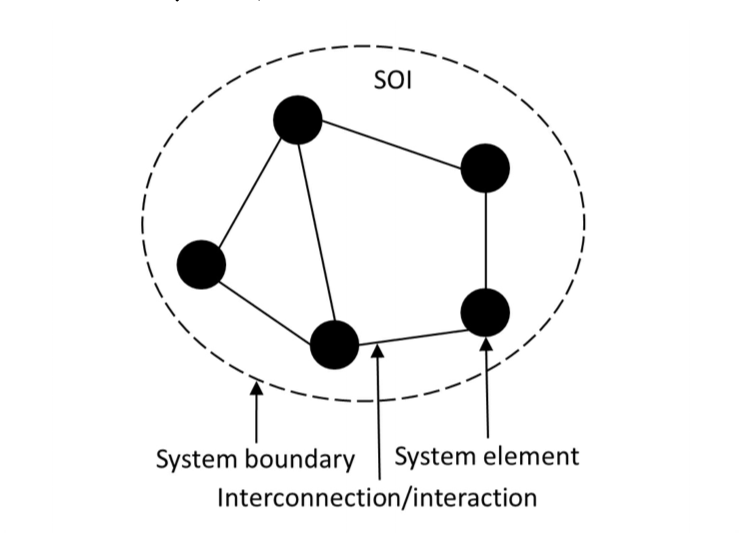
\includegraphics[height=4in]{./figures/system-of-interest.png} 
   \caption{A system of interest (SOI) \citep{{Faulconbridge2019}}}
   \label{fig:system-of-interest}
\end{figure}
Paraphrasing from \citep{Faulconbridge2019}
\begin{quote}
The purpose of the system is  called its mission.
The mission of the system is to provide a solution to a  problem. 
For a system comprised of elements that are interconnected to achieve the system?s mission, it is assumed that all three of those principal aspects result from conscious choice. 
Hence, we are referring to systems that have been deliberately designed, or engineered.
 Further, a system that has been engineered to perform a specified mission must be able to perform that mission with relative autonomy; it must be managerially and operationally independent (and may well have been procured independently).
\end{quote}
 The last aspect is called system integration -- well known integrators are Boeing, Raytheon, Microsoft. An integrator assembles components so the system performs without beneficiaries needing to be able to construct the components themselves.  We will use aspects of integration in this class to explore systems tools in engineering applications.


\section{Systems Thinking in Engineering}
Recent direction from TTU leadership is a need to instill systems thinking in courses.  
So why is such direction mandated?

\begin{quote}
As technological systems grow larger, more complex, and interdisciplinary, electronics and hi-tech industries face a growing demand for engineers with a capacity for ``engineering systems thinking.'' 
%This paper presents a multifunctional definition and 30 laws of ``engineering systems thinking''. 
%The definition and the laws are based on a study that its purpose was to identify the characteristics of engineers who are able to think in the manner called ``engineering systems thinking''. A thorough understanding of ``engineering systems thinking'' on both the theoretical and operational levels will prove useful $\dots$ 
\end{quote}
The next question is what is ``systems thinking''?

\begin{quote}``Systems thinking'', is a discipline for seeing wholes. 
It is a framework for seeing interrelationships rather than things, for seeing patterns of change rather than static ``snapshot''.
 Systems thinking offers us a flexible language that might expand, change, and shape our ordinary way of thinking in regard to complex issues.
\end{quote}

Not much of a definition but it gives some direction explicitly demanding examination beyond components into how they perform the larger mission.


Lets list some aspects of a Systems Thinking Engineer  

\begin{itemize}
\item Understanding the whole system: A problem may not be solved by breaking it down into elements and finding a separate solution for each of those elements. One must be able to see the whole picture. Some problems stem from the structure of the system itself. All system components (persons, parts) share responsibility for system problems.
Thus, an engineer with a capacity for systems thinking understands how sub-systems integrate into a whole single system and understands the whole ? the entire system and the whole picture beyond its single components.

\item Understanding the synergy of the system: The general systems theory holds that all systems are similar in certain ways. According to this view, if the synergy attribute exists in all systems, then it certainly exists in man-made technological systems. The systems engineer must, therefore, be capable of deriving the synergy of a system from the very integration of the sub-systems under his responsibility.

\item Understanding the system from multiple perspectives: A successful systems engineer would avoid adopting a one-dimensional view and would examine a specific subject or problem from different angles and points of view.

\item Understanding the implications of modification to the system: It turns out that modifications are central to the work of the systems engineer. The systems engineer must understand the system as a whole and be capable of anticipating and detailing all implications (including side effects) of changes in the system -- engineering and non-engineering alike -- both those initiated by the contractor and those required by the end user after freezing the design. In many cases, the systems engineer must be able to take care of every stage of the change starting from the conception of the idea and proceeding through the paper work (forms and approvals) and on to the execution and documentation of the introduced modification.

\item Understanding a new system immediately upon presentation: An engineer with a good grasp of the system understands and is able to describe the operation, purposes, applications, advantages, and limitations of an unknown system immediately after receiving an initial explanation.

\item System complexity level:  Dynamic complexity exists when a certain operation results in a certain series of consequences in one part of the system and a totally different series of consequences in other parts of the system. Dynamic complexity also exists when regular intervention produces results that are irregular. Regular methods of design and analysis are not structured to cope with dynamic complexity. In real life, most situations deal with dynamic complexity and not complexity of detail. Simulations with thousands of variables and complex alignments of components are likely to divert our attention from seeing the main patterns and interactions.  Thus, a system becomes more complex with the growing number of sub-systems within it, causing an increase in the number of interconnections between its components. A successful systems engineer will be better equipped to describe the functionality of complex systems.

\item Interconnections: A successful systems engineer must understand and be able to describe the interconnections (even when some of them are hidden) and the mutual influences between sub-systems (and neighboring systems).

\item Remedies for failures and system problems : Systems engineers are sometimes required to remedy/solve/analyze system failures or system problems. Engineering systems thinking a priori could, perhaps, prevent the appearance of a system failure or a system problem. Therefore the treatment of system failures/problems is a significant component of engineering systems thinking.

\item Analysis and synthesis: An engineer with a capacity for engineering systems thinking must be able to move from the whole to its parts, and analyze the system by breaking it down to its components. He or she must be able to track signals from the input through every sub-system, and interface to the output. In addition to this, however, the systems engineer must be able to synthesize. He or she must be able to assemble or connect sub-systems into a complete system and provide end-to-end solutions.

\item Don't get stuck on details: There are engineers who have to thoroughly understand all the details involved in a given problem in order to be able to form a decision and come up with a solution. Engineers of this sort usually find it difficult to develop engineering systems thinking. A successful systems engineer must be able to see the whole picture and not get stuck on details. He or she should be able to act without understanding fully all of the system's details. Such engineers usually feel comfortable working in unclear conditions and in an uncertain environment.

\item Multidisciplinary and interdisciplinary knowledge: The single most prominent characteristic of an engineer with a capacity for engineering systems thinking is multidisciplinary knowledge, as well as interdisciplinary knowledge. Knowledge of this sort makes one comfortable with multi-tasking activities. Multidisciplinary knowledge does not mean that one knows a little of everything. The systems engineer must acquire specialization in at least one main area (an anchor); in addition, he or she must be knowledgeable in all other relevant areas.  The engineer's knowledge in those other areas need not be equal to that of a specialist. In the additional content areas, the systems engineer must possess general knowledge and understanding on the overall level. He or she must be familiar with the jargon of the other disciplines (relevant to his occupation and tasks), and be able to communicate with people from different areas. Wide knowledge is required for the systems engineer also in order to be able to understand and derive significance from the answers and reports of others, i.e. ?specialists? from outside his own main area of expertise. Such wide knowledge may also enable the systems engineer to cope with new disciplines.
\end{itemize}

Some of these are kind of bullshit -- we can identify that as we proceede but in general the list simply  calls for accepting complexity and uncertainty.
A further expansion of these concepts is listed in a set of systems laws \citep{Frank2002} listed below
\begin{enumerate}
\item In all the project's phases/stages and along the system's life, the systems engineer has to take into account the customer organization vision, goals and tasks, the customer requirements and preferences, and the problems to be solved by the system and the customer needs.
\item The whole has to be seen as well as the interaction between the system's elements. For this purpose a circular thinking has to be developed, to replace the traditional linear thinking. A problem should not be solved by just dismantling it to parts but all its implications have to be taken into account. Each activity in a system's certain element affects the other elements and the whole.
\item Consider that every action could have implications also in another place or at another time.
\item One should always look for the synergy and the relative advantages stemming from the integration of sub-systems.
\item The solution is not always only engineering one. The systems engineer has also to take into account cost, re-use, organizational, managerial, and personal considerations.
\item The system's engineer should take as many different perspectives as possible, of every subject or problem, and other aspects have to be reviewed from all points of view.
\item Always take into account electrical considerations, mechanical considerations, environmental conditions constraints, quality assurance considerations, and benefit indices, such as reliability, availability, maintainability, testability and productibility.
\item In all development phases the future logistic requirements have to be taken into account (spare parts, maintenance infrastructures, support, service, maintenance levels, worksheets, technical documentation and various manuals).
\item When a need arises to carry out a modification in the system, take into account: the engineering and non-engineering implications in any place and at any time; the effects on the Form, Fit and Function; the delays and the time durations of the modification incorporation; the system's response time to the changes; the needs, difficulties and attitudes of those supposed live with the modification; that the change could bring short-term benefit but long-term damage.
\item Each problem may have more than one possible working solution. All possible alternatives should be examined and compared to each other by quantitative and qualitative measurements. The optimal alternative should be chosen.
\item Engineering design is not necessarily maximal. One should not always aspire to achieve maximum performances. At every stage engineering trade-offs and cost-effectiveness considerations should be considered. One could always improve more. One has to know when to ?cut? and freeze a configuration for production. Excessive pressure in a certain point could cause a collapse at another point. Over stressing one part in the system could weaken another part and thus the entire system. Maximum performance design is expensive and not always results in maximizing entire system performance.
\item In case of system's malfunction, problem or failure, repeated structures and patterns should be looked for and analyzed, and lessons drawn accordingly (repeated failure is a failure that keeps returning, after the repairs, until the true malfunction is found and repaired. A repeated-non-verified failure is a failure that the user complained about, the technician inspected and could not verify and the failure reappeared again in the next operation).
\item Look always for the leverage point ? changes that might introduce significant improvements by minimum effort.
\item Pay attention to and take into account slow or gradual processes.
\item Avoid adapting a known solution for the current problem ? it might not be suitable.
\item Take into account development risks. In each project uncertainty prevails on the level of scheduling, cost, resources, scope, environmental conditions and technology. Therefore, the strategy of eliminating uncertainties has to be taken ? e.g. experiments, tests, verifications, analyses, comparisons, simulations, awareness of possible risks, planning ways of retreat and risk deployment among the partners.
\item It is impossible to run a project without control, configuration management, milestones and management and scheduling methods. Possible bottlenecks and potential critical paths have to be examined constantly.
\item The operator/user person must be considered as major part of the system. Hence at each stage, the human element has to be considered. The engineering design should include MMI (Man-Machine-Interface) considerations.
\item The engineering design is a top-down design (excluding certain ?open systems?, for which the bottom-up approach is preferable). The integration and tests are bottom-up.
\item At every stage, systemic design considerations should be used (such as decentralized or centralized design, minimum dependency between sub-systems, etc.). The systems engineer should be familiar with system malfunction analysis methods and tools.
\item Engineering systems thinking requires the use of simulations. The simulation limitations should be taken into account.
\item Engineering systems thinking requires the integration of expertise from different disciplines. As the systems become more complex and dynamic, one person, as competent as he may be, is inadequate to understand and see it all. Systems thinking, by its nature requires the examination of different perspectives, calling for teamwork to cover the various perspectives. When setting up the team proper representation has to be given to all the system's functions. Control and status discussions and meetings as well as ?brain storming? may have to be more frequent.
\item Try to anticipate the future at every stage. Take into account anticipated technological developments, future market needs, difficulties, problems and expected changes in the project.
\item Selecting partners and sub-contractors could be critical. Before signing agreements refer to considerations such as the ?engineering/economic history? of the potential partner, manpower (quality, stability, human capital) that he is capable of investing at the project's disposal, division of work and responsibility and proper arrangements for status meetings, integration tests and experiments of all kind.
\item When selecting the software language or software development tools and platforms, make sure that they are usable and supportable, or changeable, throughout the system's life.
\item When selecting components for production, take into account their shelf life. Select components whose supply is guaranteed throughout all the system's life. In case of likely obsolescence of component, make sure of having sufficient stock.
\item In order to win a tender, many companies reduce the development price in their offer, assuming that they will be compensated by the serial production and by the cost of modifications (if required). Therefore, in engineering systems thinking, it is recommended not to start development at all, if the serial production budgets are not guaranteed in advance.
\item Always examine the external threats against the system (for example, electro-magnetic-interference, environment conditions, etc.).
\item Engineering systems thinking resorts probability and statistical terms, both when defining the system specifications and when determining the project targets (costs, performance, time and scope).
\item In engineering systems thinking it is advisable to limit the responsibility assigned to an external factor (such as external counselor), since this increases the dependency on it.
\end{enumerate}

\section{Components Integration }
Integration of components is where I think the real action occurs, and this course will focus on this aspect.


\begin{thebibliography}{9}

%\bibitem[Asquith (2002)]{AsquithRegulation2002}
%Asquith, W.H., 2002, Effects of Regulation on L-moments of Annual Peak Streamflow in Texas.
%U.S. Geological Survey Water Resources Investigations Report 01--4243,
%\url{https://pubs.usgs.gov/wri/wri014243/pdf/wri01-4243-new.pdf}

\bibitem[Faulconbridge (2019)]{Faulconbridge2019}
Faulconbridge, Ian. Introduction to Systems Engineering (Kindle Location 181). Argos Press Pty Ltd. Kindle Edition. 

\bibitem[Frank (2002)]{Frank2002}
Frank, M. (2002), ``What is ``engineering systems thinking''?'', Kybernetes, Vol. 31 No. 9/10, pp. 1350-1360. \url{https://doi.org/10.1108/03684920210443554}
\end{thebibliography}

\end{document}